\documentclass[letter,11pt]{article}

\usepackage[spanish,es-nodecimaldot]{babel}
\usepackage[utf8]{inputenc}

\usepackage{lmodern}
\usepackage[T1]{fontenc}
\usepackage{textcomp}

\usepackage{framed}
\usepackage[svgnames]{xcolor}
\colorlet{shadecolor}{Gainsboro!50}

\usepackage[shortlabels]{enumitem}
\usepackage{graphicx}
\usepackage{pstricks}

\usepackage{anysize}
\marginsize{3cm}{2cm}{2cm}{3cm}

\usepackage{siunitx}
\usepackage{amsmath}
\usepackage{array}
\usepackage{alltt}

\usepackage{fancyhdr}
\usepackage{lastpage}
\pagestyle{fancy}
\fancyhf{}
\fancyhead[LE,RO]{Física Básica III}
\fancyfoot[CO,CE]{\thepage\ de \pageref{LastPage}}

\special{papersize=215.9mm,279.4mm}

\usepackage[
    pdfauthor={Carlos Eduardo Caballero Burgoa},%
    pdftitle={Física Básica III},%
    pdfsubject={Tarea 02},%
    colorlinks,%
    citecolor=black,%
    filecolor=black,%
    linkcolor=black,%
    urlcolor=black,
    breaklinks]{hyperref}
\usepackage{breakurl}

\newcommand{\blankpage}{
\newpage
\thispagestyle{empty}
\mbox{}
\newpage
}

\renewcommand{\arraystretch}{1.2}

\begin{document}

\begin{center}
    {\Large \bf{\underline{Tarea \#02}}}
\end{center}
\vspace{0.5cm}

\textbf{21.57.}
Tres cargas se encuentran en los vértices de un triángulo isósceles como
se muestra en la figura. Las cargas de $\pm 5.00 \mu C$ forman un dipolo.

\begin{figure}[!h]
\centering
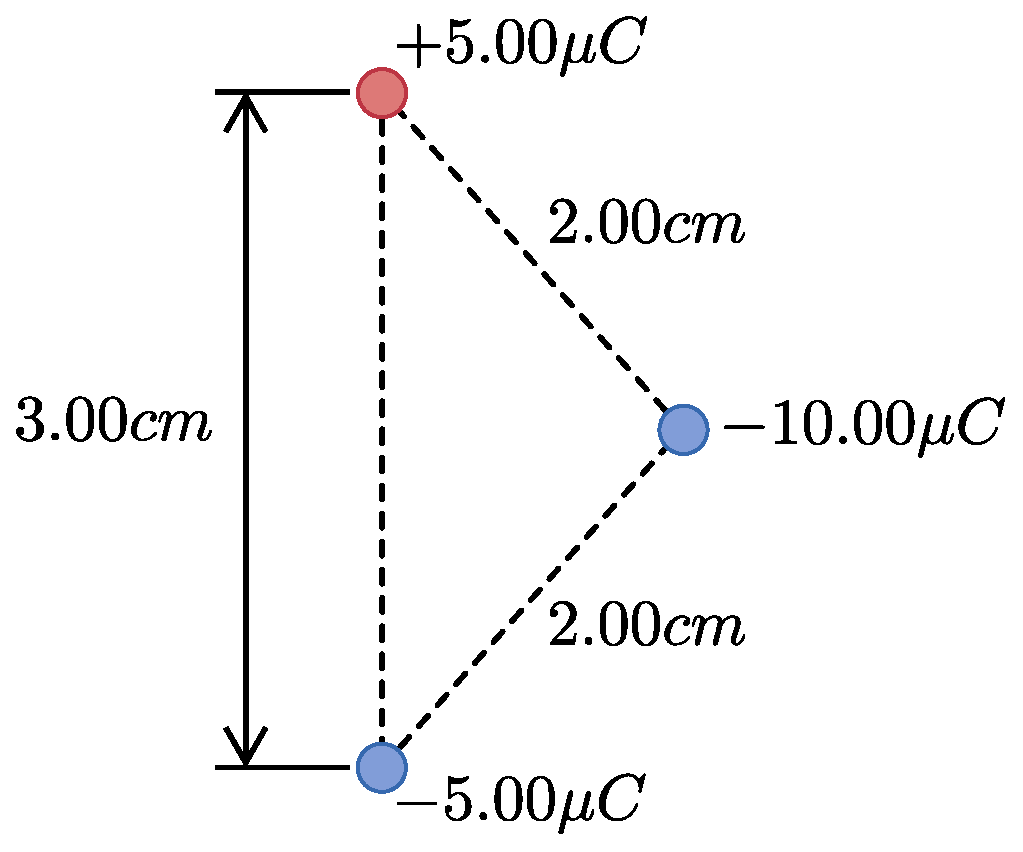
\includegraphics[scale=0.32]{resources/f1.eps}
\end{figure}

\begin{enumerate}[a)]
\item Determine la fuerza (magnitud y dirección) que la carga de $-10.00 \mu C$
ejerce sobre el dipolo.
\item Para un eje perpendicular a la línea que une las cargas de
$\pm 5.00 \mu C$ en el punto medio de dicha línea, obtenga el par de torsión
(magnitud y dirección) ejercido sobre el dipolo por la carga de $-10.00 \mu C$.
\end{enumerate}

\vspace{0.5cm}
\textbf{\underline{Solución}:} \\

Los vectores de posición de las cargas son:

\begin{equation*}
    \vec{r} = 0.025 \hat{u}_x + 0.015 \hat{u}_y [m]
\end{equation*}

\textbf{21.78.}
Un objeto pequeño de masa $m$, carga $q$ y rapidez inicial
$v_0 = \num{5.00e3} [m/s]$ se proyecta hacia un campo eléctrico uniforme entre
dos placas metálicas paralelas con longitud de $26.0 [m]$ (figura).
El campo eléctrico entre las placas está dirigido hacia abajo y tiene una
magnitud $E = 800 [N/C]$. Suponga que el campo es igual a cero afuera de la
región entre las placas. La separación entre las placas es lo suficientemente
grande para que el objeto pase entre ellas sin golpear la placa inferior.
Después de pasar por la región del campo, el objeto se curva hacia abajo una
distancia vertical $d = 1.25 [cm]$ a partir de la dirección original del
movimiento y alcanza una placa recolectora que está a $56.0 [cm]$ del extremo
de las placas paralelas. Ignore la gravedad y la resistencia del aire. Calcule
la razón carga-masa $q/m$ del objeto.

\begin{figure}[!h]
\centering
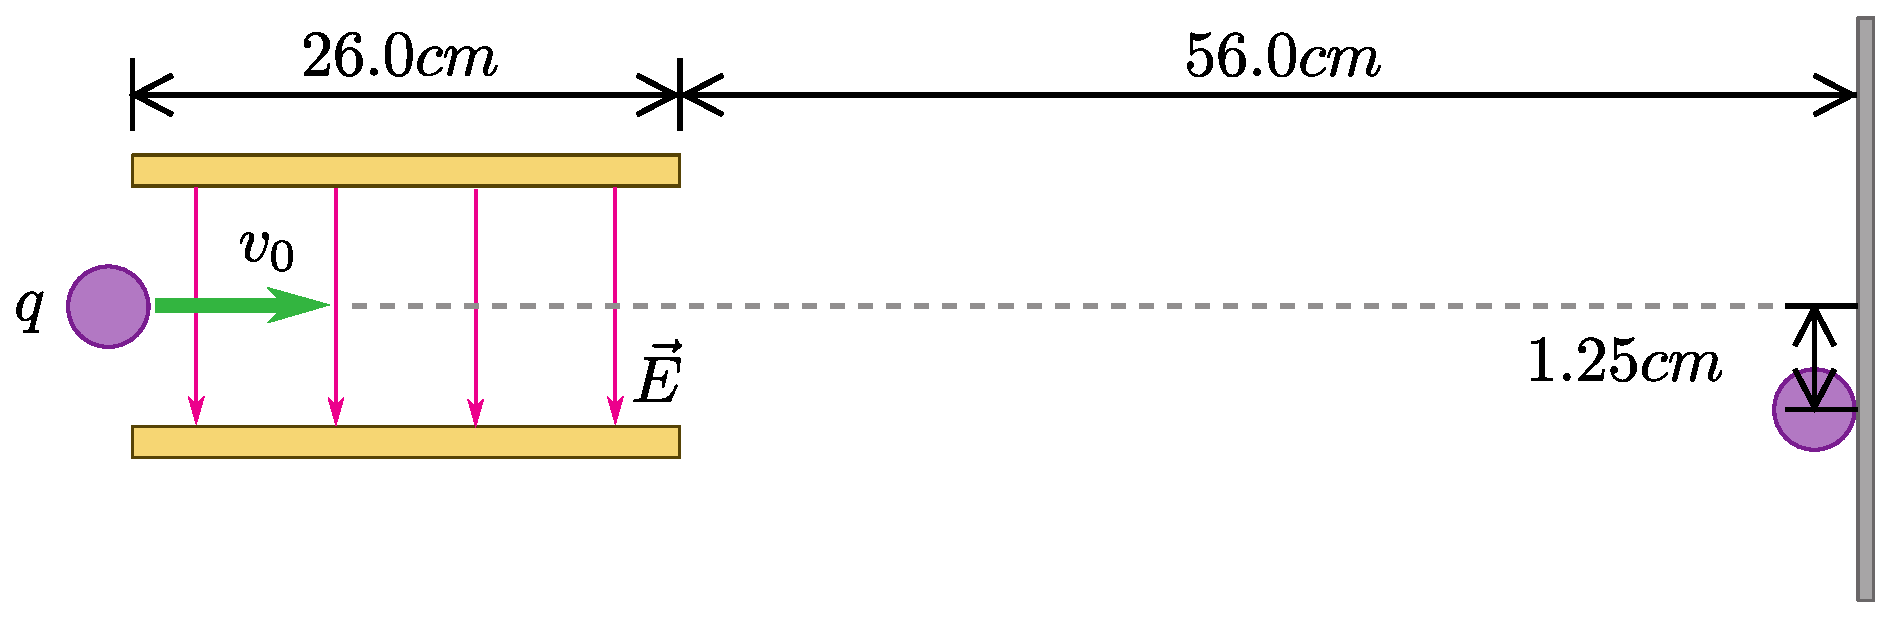
\includegraphics[scale=0.35]{resources/f2.eps}
\end{figure}

\vspace{0.5cm}
\textbf{\underline{Solución}:} \\

Los vectores de posición de las cargas son:

\begin{equation*}
    \vec{r} = 0.025 \hat{u}_x + 0.015 \hat{u}_y [m]
\end{equation*}

\textbf{21.95.}
Tres cargas se colocan como se ilustra en la figura. La magnitud de $q_1$ es
$2.00 \mu C$, pero no se conocen el signo ni el valor de la carga $q_2$. La
carga $q_3$ es de $+4.00 \mu C$, y la fuerza neta $\vec{F}$ sobre $q_3$ está
por completo en la dirección negativa del eje $x$.

\begin{enumerate}[a)]
\item Considere los diferentes signos posibles de $q_1$ y que hay cuatro
posibles diagramas de fuerza que representan las fuerzas $\vec{F_1}$ y
$\vec{F_2}$ que $q_1$ y $q_2$ ejercen sobre $q_3$. Dibuje esas cuatro
configuraciones de fuerza posibles.
\item Con el empleo de los diagramas del inciso a) y la dirección de $\vec{F}$,
deduzca los signos de las cargas $q_1$ y $q_2$.
\item Calcule la magnitud de $q_2$.
\item Determine $\vec{F}$, la magnitud de la fuerza neta sobre $q_3$.
\end{enumerate}

\begin{figure}[!h]
\centering
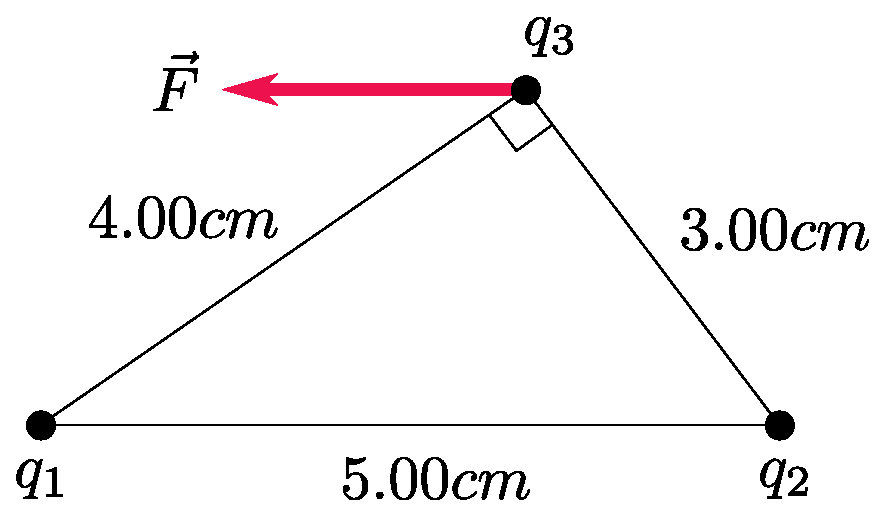
\includegraphics[scale=0.34]{resources/f3.eps}
\end{figure}

\vspace{0.5cm}
\textbf{\underline{Solución}:} \\

a)
\begin{figure}[!h]
\centering
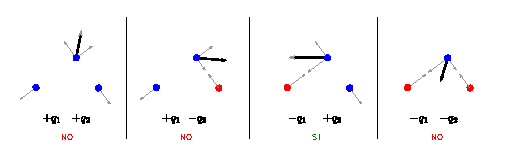
\includegraphics[scale=1.90]{resources/f3.1.eps}
\end{figure}

b)
Para que $\vec{F}$ se dirija horizontalmente, las cargas deben ser $-q_1$ y
$+q_2$.

c)
Los vectores de posición de las cargas son:

\begin{equation*}
    \vec{r} = 0.025 \hat{u}_x + 0.015 \hat{u}_y [m]
\end{equation*}

\end{document}

